\documentclass[12pt,a4paper,titlepage]{article}
\usepackage[utf8]{inputenc}
\usepackage{setspace}
\usepackage{enumitem}
\usepackage{authblk}
\usepackage[UKenglish]{datetime}
\usepackage{listings}
\usepackage{xcolor}
\usepackage{bera}
\usepackage[letterpaper, portrait, margin=1.2in]{geometry}
\usepackage[linguistics]{forest}
\usepackage{hyperref}

\lstdefinestyle{mystyle}{
keywordstyle=\color{blue}
}
\lstset{style=mystyle}

\date{}
\newdateformat{ndate}{\THEDAY~\monthname[\THEMONTH], \THEYEAR}

\newdimen\origiwspc
\newdimen\origiwstr
%\newenvironment{fontspace}[2]
%

\begin{document}

\begin{titlepage}
\vspace*{\fill}
\begin{center}
\centering
\begin{Huge}
{\textbf{\bfseries eBook Maker\\}}
\huge CS699 Software Lab Project\\
\LARGE Indian Institute of Technology, Bombay\vspace{8mm}\\
We\_did\_our\_best\vspace{4mm}\\
\end{Huge}
\begin{large}
{Sanjna Mohan - 20305R006\\
Manjusree M P - 203059007\\
Pooja Gayakwad - 203050076\\
Snehlata Yadav - 203050075\\}
\end{large}
\vspace{0.5cm}
\begin{Large}
18\textsuperscript{th} November, 2020
\end{Large}
\author{}
\end{center}
\vspace*{\fill}
\end{titlepage}

\tableofcontents

\newpage
%\begin{fontspace}{1.5}{2}

\section{\textbf{Introduction}}
Sometimes we need content regarding some technology or topic which is distributed among multiple pages in a website, and it is quite a task in itself to go through all the links and download them. To ease the process of collecting all the related content at one place, we came up with this project. Our solution is a GUI application that takes the particular URL from the user as input, and use web scraping to get the contents as a centralized epub document which can be saved at our convenience.
\section{\textbf{Motivation}}
While going through vast tutorials on the web, sometimes it becomes tedious to go to all the links and read.
Moreover, the availability only in the presence of Internet makes it difficult for future reference.
We have come up with this project to ease the process and to download the tutorial onto our computers as an eBook.
This way, not only we get the contents in an organized manner, but also we can avail it as and when we require.
Our solution is a GUI application that takes the particular URL from the user as input, and use web scraping to get the contents as a centralized epub document which can be saved at our convenience.
\section{\textbf{User Documentation}}
\subsection{\textbf{Dependencies}}
Make sure you have the following libraries installed on your system:
\begin{itemize}
    \item tqdm
    \item BeautifulSoup
    \item ebooklib
    \item Pillow
    \item requests
\end{itemize}
Please note that this is a \textbf{Windows} application.
\subsection{\textbf{eBook Maker Usage}}
To begin with using the eBook Maker, clone the repository onto your system:
\newline 

\textbf{git clone https://sanjnamohan@git.cse.iitb.ac.in/sanjnamohan/eBookmaker.git}
\newline 
\newline \textbf{NOTE}: Do not change the directory structure after cloning.
\newline Before proceeding further, make sure you have Python installed on your system.
\newline To install Python for Windows : \url{https://www.python.org/downloads/windows/}
To install/upgrade pip : \url{https://pip.pypa.io/en/stable/installing/}
\newline
\\Go inside the folder "eBookmaker/source". 
\newline
\\Make sure the relevant libraries are installed, by running the following command on the terminal:
\newline 

\textbf{pip install -r requirements.txt}
\newline \\You are now ready to use the eBook Maker.The procedure to run the GUI application is as follows:
\begin{enumerate}
\item Double click on epub.exe and wait for few seconds till the GUI appears.
\\\newline \textbf{(OR)} \newline\\
The source code is available in epub.py. To execute directly from the source, run:
\newline 

\textbf{python epub.py}
\\
\\
\newpage
\item Once the GUI appears, enter the URL of which the document is to be created.
\newline \\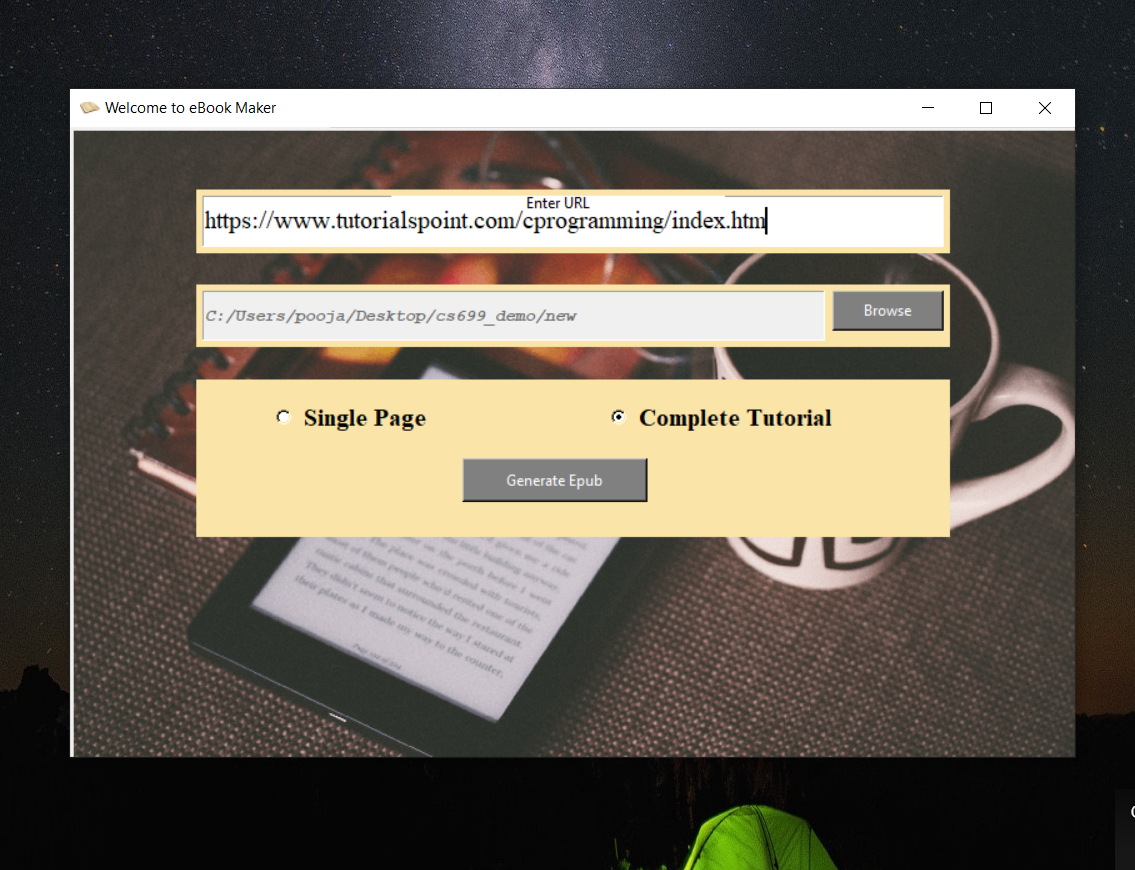
\includegraphics[width=\textwidth,height=8.5cm]{1.png}
\newline 
\item Select the destination folder using "Browse" button.
\newline \\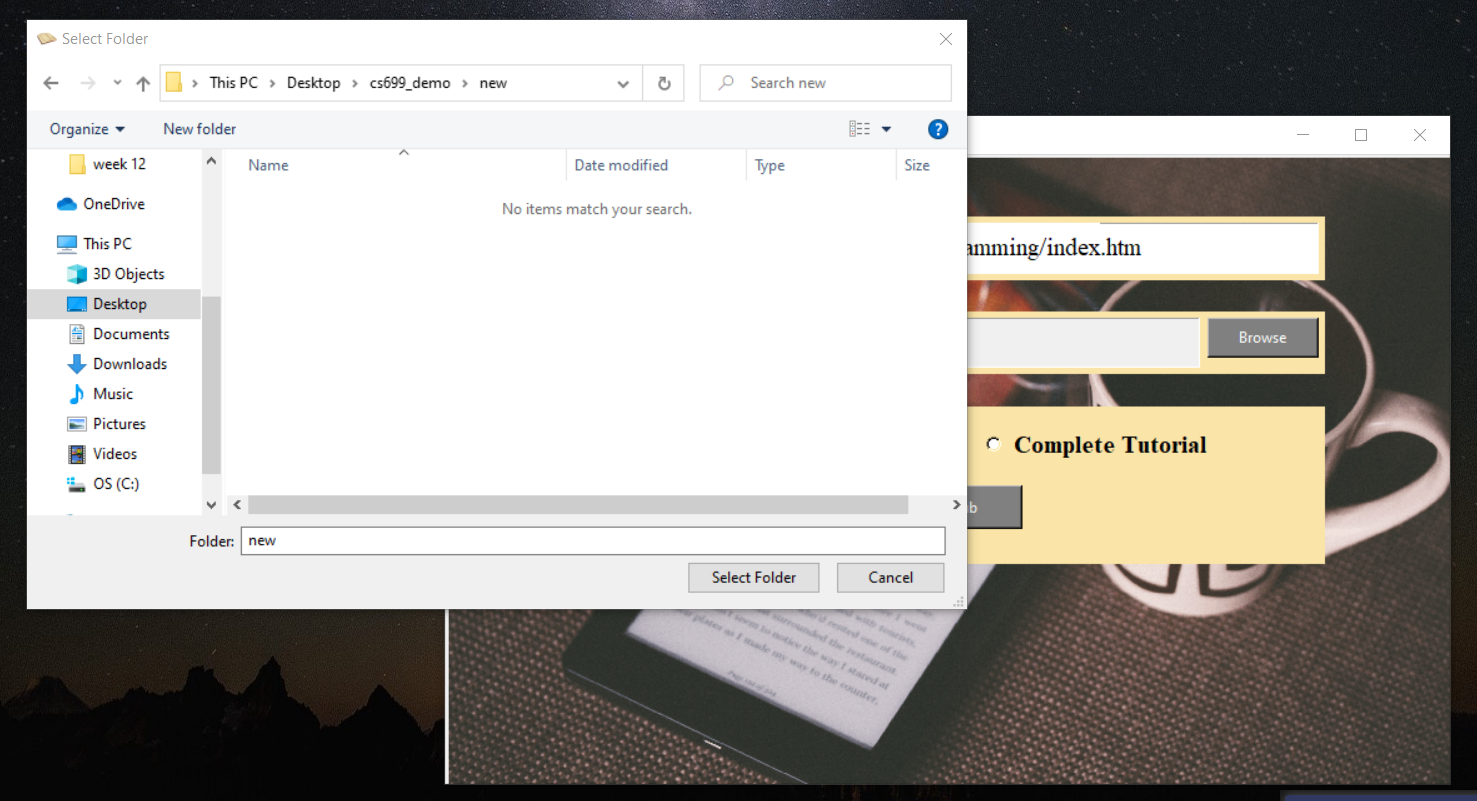
\includegraphics[width=\textwidth,height=8.5cm]{2.png}
\newline 
\newpage
\item Select either of "Single Page" or "Complete Tutorial" radio buttons and click "Generate Epub" button.
\newline \\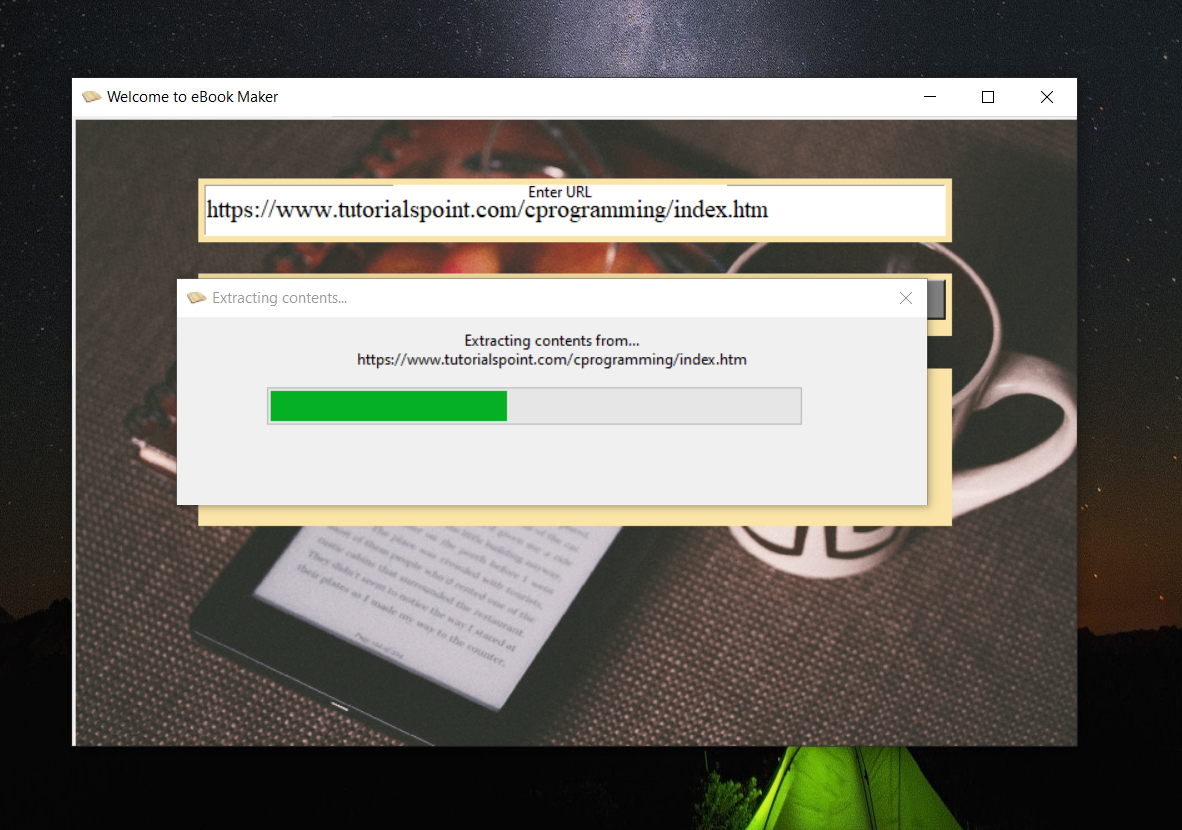
\includegraphics[width=\textwidth,height=8.5cm]{3.png}
\newline 
\item The generated eBook would be present at the set destination folder.
\newline \\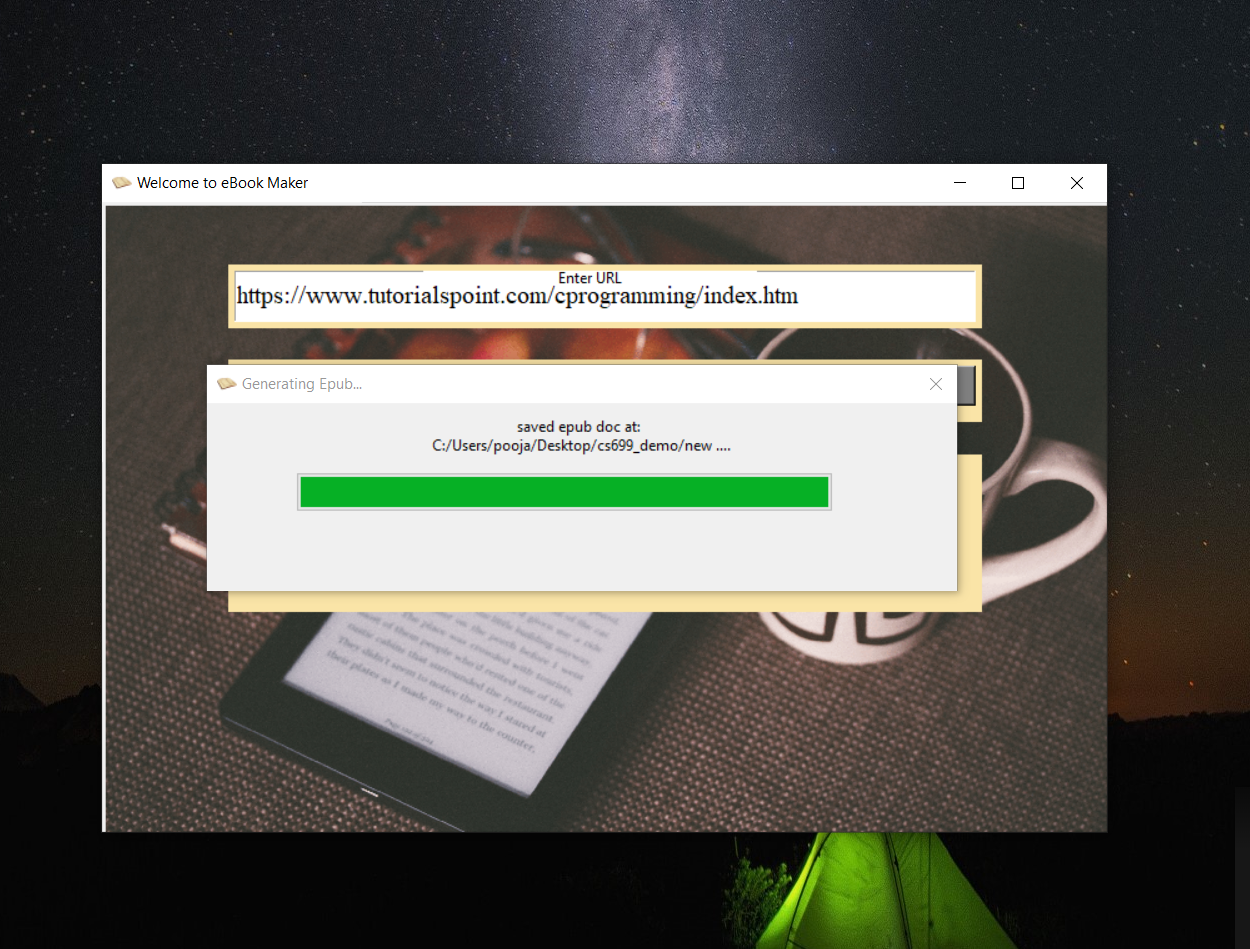
\includegraphics[width=\textwidth,height=8.5cm]{4.png}
\newline 
\newpage
\item The epub document can be read whenever required:
\newline \\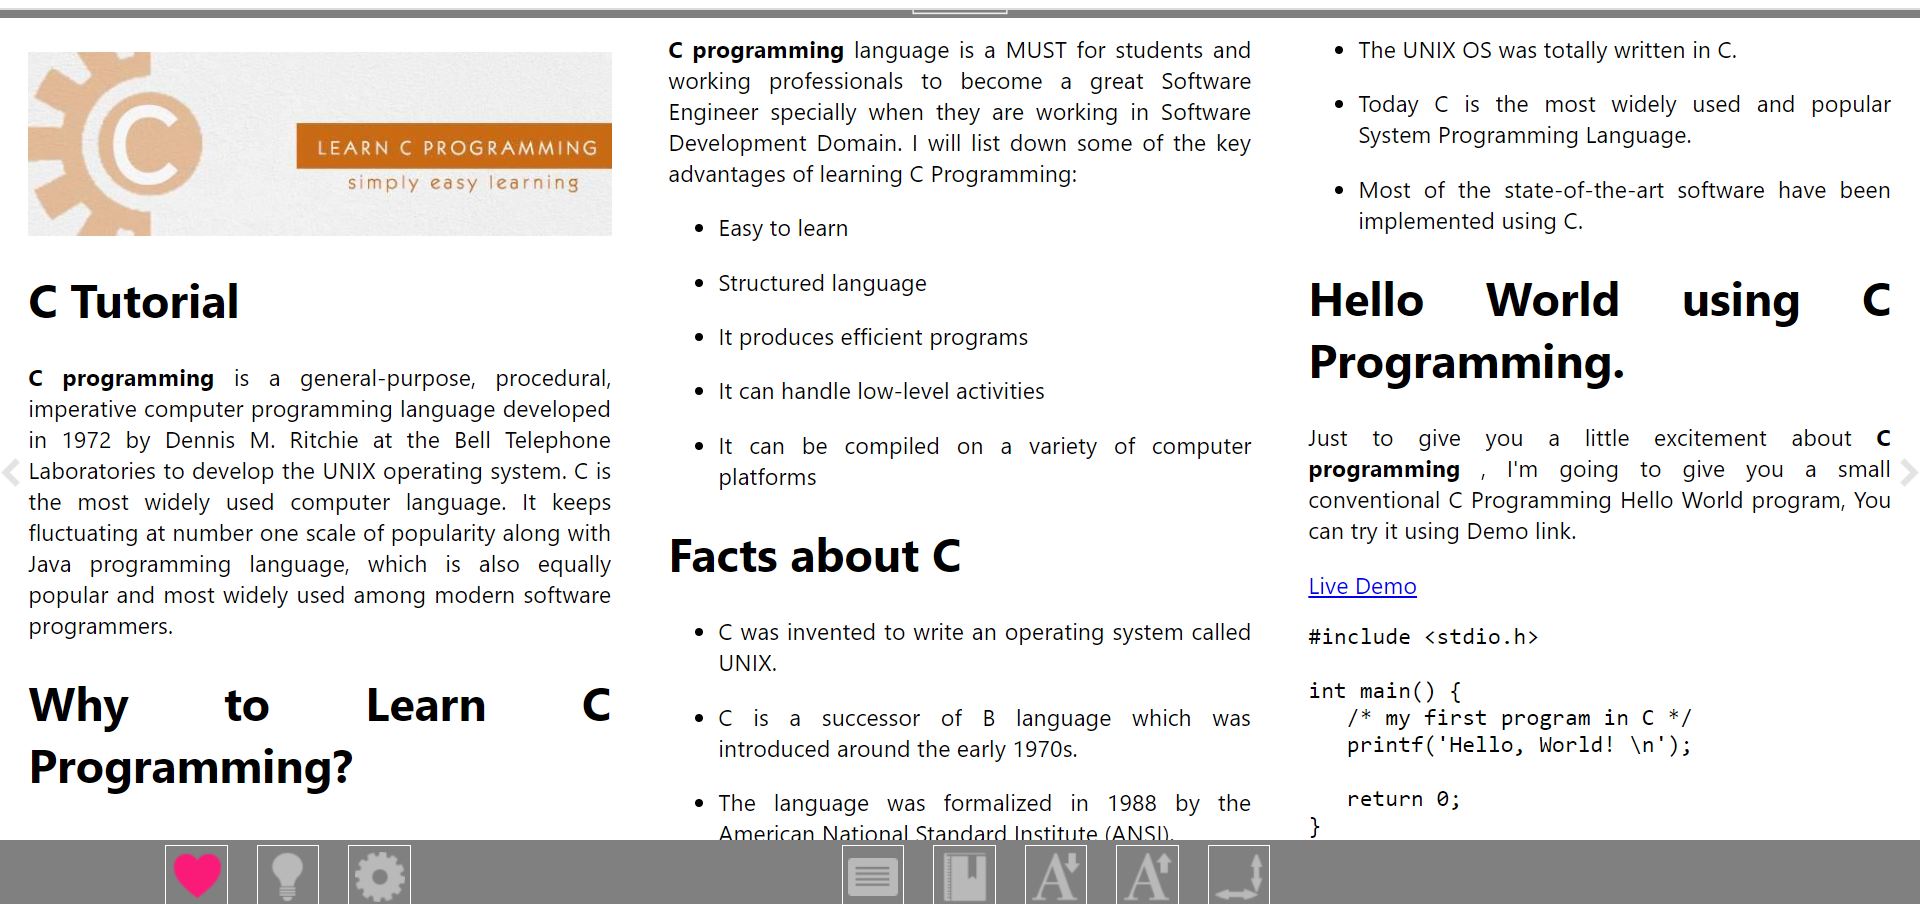
\includegraphics[width=\textwidth,height=8.5cm]{5.png}
%\end{fontspace}
\end{enumerate}
\section{\textbf{Relevance and Future Scope}}
eBook Maker is helpful in the easy compilation of tutorials from the web onto our local systems, which can be referred whenever required. The fact that eBooks can be easily shared is an added advantage. \\

eBook Maker currently works for the following links:
\begin{itemize}
    \item Tutorial topics in \url{https://www.tutorialspoint.com/}
    \item \url{https://www.geeksforgeeks.org/c-programming-language/} and other tutorial topics in geeksforgeeks
    \item \url{https://numpy.org/doc/stable/user/quickstart.html}
    \item \url{https://docs.python.org/3/tutorial/}
\end{itemize}
This can be extended to include more relevant tutorial sites. Ultimately, the aim would be to upgrade the application such that it can extract content from any website that has useful public content in it. 
\\Another important future extension would be to make it platform independent, for now it is a Windows application.
\end{document}